% !TEX TS-program = pdflatex
% !TEX encoding = UTF-8 Unicode

% This is a simple template for a LaTeX document using the "article" class.
% See "book", "report", "letter" for other types of document.

\documentclass[11pt]{article} % use larger type; default would be 10pt

\usepackage[utf8]{inputenc} % set input encoding (not needed with XeLaTeX)
\usepackage{amsmath}
\usepackage{graphicx}
\graphicspath{ {./} }
%%% Examples of Article customizations\textbf{}
% These packages are optional, depending whether you want the features they provide.
% See the LaTeX Companion or other references for full information.

%%% PAGE DIMENSIONS
\usepackage{geometry} % to change the page dimensions
\geometry{a4paper} % or letterpaper (US) or a5paper or....
% \geometry{margin=2in} % for example, change the margins to 2 inches all round
% \geometry{landscape} % set up the page for landscape
%   read geometry.pdf for detailed page layout information

\usepackage{graphicx} % support the \includegraphics command and options
\usepackage{physics}

% \usepackage[parfill]{parskip} % Activate to begin paragraphs with an empty line rather than an indent

%%% PACKAGES
\usepackage{booktabs} % for much better looking tables
\usepackage{array} % for better arrays (eg matrices) in maths
\usepackage{paralist} % very flexible & customisable lists (eg. enumerate/itemize, etc.)
\usepackage{verbatim} % adds environment for commenting out blocks of text & for better verbatim
\usepackage{subfig} % make it possible to include more than one captioned figure/table in a single float
\usepackage{fancyvrb}
\usepackage{hyperref}
\usepackage{listings}

% These packages are all incorporated in the memoir class to one degree or another...

%%% HEADERS & FOOTERS
\usepackage{fancyhdr} % This should be set AFTER setting up the page geometry
\pagestyle{fancy} % options: empty , plain , fancy
\renewcommand{\headrulewidth}{0pt} % customise the layout...
\lhead{}\chead{}\rhead{}
\lfoot{}\cfoot{\thepage}\rfoot{}

%%% SECTION TITLE APPEARANCE
\usepackage{sectsty}
\allsectionsfont{\sffamily\mdseries\upshape} % (See the fntguide.pdf for font help)
% (This matches ConTeXt defaults)

%%% ToC (table of contents) APPEARANCE
\usepackage[nottoc,notlof,notlot]{tocbibind} % Put the bibliography in the ToC
\usepackage[titles,subfigure]{tocloft} % Alter the style of the Table of Contents
\renewcommand{\cftsecfont}{\rmfamily\mdseries\upshape}
\renewcommand{\cftsecpagefont}{\rmfamily\mdseries\upshape} % No bold!

%%% END Article customizations

%%% The "real" document content comes below...

\title{Mining Bitcoin Using Grover's Algorithm}


\author{Shazil Arif}
%\date{} % Activate to display a given date or no date (if empty),
         % otherwise the current date is printed 

\begin{document}
\maketitle

\tableofcontents

\section{Introduction}{}

In this paper we cover the basics of Bitcoin, Blockchain and Bitcoin's Proof-of-Work Consensus Algorithm and explore what mining is. We will discuss why mining is difficult and the existing solutions that exist for it. Then we will look at how we can attempt to solve it (at a very small scale) using Grover's Algorithm.\\


\noindent \textbf{Disclaimer:} I'm not an expert in any of the topics discussed in this paper.

\section{Blockchain}{}

A blockchain is simply a ledger. It records transactions. It records the sender, receiver and the amount being sent by the sender to the receiver. It's a concept that has been around for thousands of years.\\

\noindent In ancient times, in places like Babylon and Mesopotamia, people used clay tablets and carved details of transactions onto these tablets. Slowly these evolved into papyrus documents. In the 1t5h century, italian mathematician Luca Pacioli introduced the idea of double entry bookkeeping. It became the underlying principle of today's field of accounting. It's very simple, each transaction involves a credit entry for one party and a debit entry for another party.\\

\noindent Blockchain is essentially a modern versional of a ledger. It is digital but also \textbf{decentralized}. We'll discuss the concept of decentralization more in depth but, at a high level what it means is that nobody owns or controls the ledger. In ancient times, ledgers were stored in temples, then banks in more modern times. Instead, the blockchain is stored on various computers referred to as a network.\\

\noindent Blockchain is in fact not tied to Bitcoin. It was invented years before Bitcoin by Stuart Haber and W. Scott Stornetta who worked at Bell labs in 1991. Their motivation was to create a way of making digital documents immutable and tamper-proof. \\

\noindent In technical terms, a blockchain is implemented as a distributed database. The database structures data into blocks and links them together, creating a chain of blocks. Each block contains a set of transactions and is assigned a hash. The hash is a combination of multiple details including sender, receiver, transactions etc.  but most importantly, the hash of the previous block. Each block contains the hash of the block before it. For example, Block 2 would have the hash of Block 1. This is important, because if someone tries to tamper with Block 1, it's hash would change but, Block 2 contains Block 1's hash which would also become invalid and a result, the hash of Block 2 would become invalid. If there are more blocks, Block 3, 4 and so on, al of theml become invalid. This is very powerful as it makes a blockhain highly tamper proof. Attempting to tamper one block, invalidates all the others. \\

\section{Currency and Cryptocurrencies}{}
What is a cryptocurrency? How does it have value if I can't see or feel it? A question many people commonly ask.\\


\noindent Fundamentally, nowadays most currencies (digital or paper) have no value. It has value because society agreed that it will be used as a medium of exchange and a result, has value. It is a social construct. This is known as the Fiat Standard. It's worth pointing out that this wasn't always the case. Before 1971, the US dollar and many currencies around the world were backed gold, a physical asset. It was known as the Bretton Wood System or Agreement. However, in August 1971, President Richard Nixon broke this agreement in order to fight unemployment, inflation and stabilize the US dollar. The US dollar was no longer backed by gold and many other countries followed.\\


\noindent Most Cryptocurrencies (including Bitcoin) are also technically fiat currencies. They are not backed by anything and they only have value because the people using agreed upon them as a medium of exchange. However, there are other factors that play a role in determining the value of a currency. We'll discuss these factors, specifically for Bitcoin in the next section. In addition, these currencies live on a Blockchain that is secured via cryptographic hash functions, which is where the name comes from. Cryptography + currency = Cryptocurrency\\

\section{Bitcoin}{}
\subsection{Overview}{}
As we discussed earlier, Bitcoin is a cryptocurrency. It was introduced to world in the famous white paper titled \textbf{Bitcoin: A Peer-to-Peer Electronic Cash System} published by Satoshi Nakamoto on October 31, 2008, not long after the 2008 financial collapse. What Satoshi really wanted was: decentralized currency, one that was truly controlled by no bank or third party. Instant online transfers, and make all of that secure.

\subsection{Price Factors}{}
\subsection{Byzantine General's Problem and Consenus}{}
It's worth pointing out that Bitcoin did not solve the problem of online money transfers or creating tamper proof ledgers, these were solved problems before Bitcoin came around. Bitcoin drew heavily on earlier works in cryptography and digital security (more on this later). What Satoshi really solved was the problem of Consensus. At a high level, the problem was: In a distributed system, how do different nodes agree on the state of the blockchain.
\subsection{The Bitcoin Network and distributed Nodes}{}
\subsection{Cryptography and security}{}
\subsection{Public Adoption}{}
\subsection{Environmental Impact}{}


\section{Proof-of-Work and Mining}{}
\subsection{A brief history of Proof of Work}
\subsection{Overview}
\subsection{Hashing and the search for a nonce}
\subsection{Mining Technology}


\section{Grover's Algorithm}{}
Grover's Algorithm is a quantum search algorithm. It can search an unsorted list of items in $O(\sqrt{N})$ evaluations of the oracle function. It uses a technique called amplitude amplification that repeatedly applies the algorithm and with each iteration, our target result has a higher and higher probability. Essentially, we are amplifying results of interest.\\

\noindent Suppose we have $N = 2^{n}$ possible states, where $n$ is the number of bits. We start by defining a Unitary matrix $U_w$. Then we do the following:

\begin{itemize}

\item[1)] Initialize the system to the uniform superposition over all states:\\

$ \ket{s} = \frac{1}{\sqrt{N}}  \sum_{x = 0}^{N - 1} \ket{x}$

\item[2)] Perform the following $k$ times ($k$ is about $\frac{\pi}{4} \sqrt{N)}$:

\begin{itemize}
\item[1)] Apply the operator $U_w$
\item[2)] Apply the Grover diffusion operator $U_s = 2 \ket{s} \bra{s} - I$
\end{itemize}
\item[3)] Measure results
\end{itemize}

The circuit looks as follows:\\

\noindent 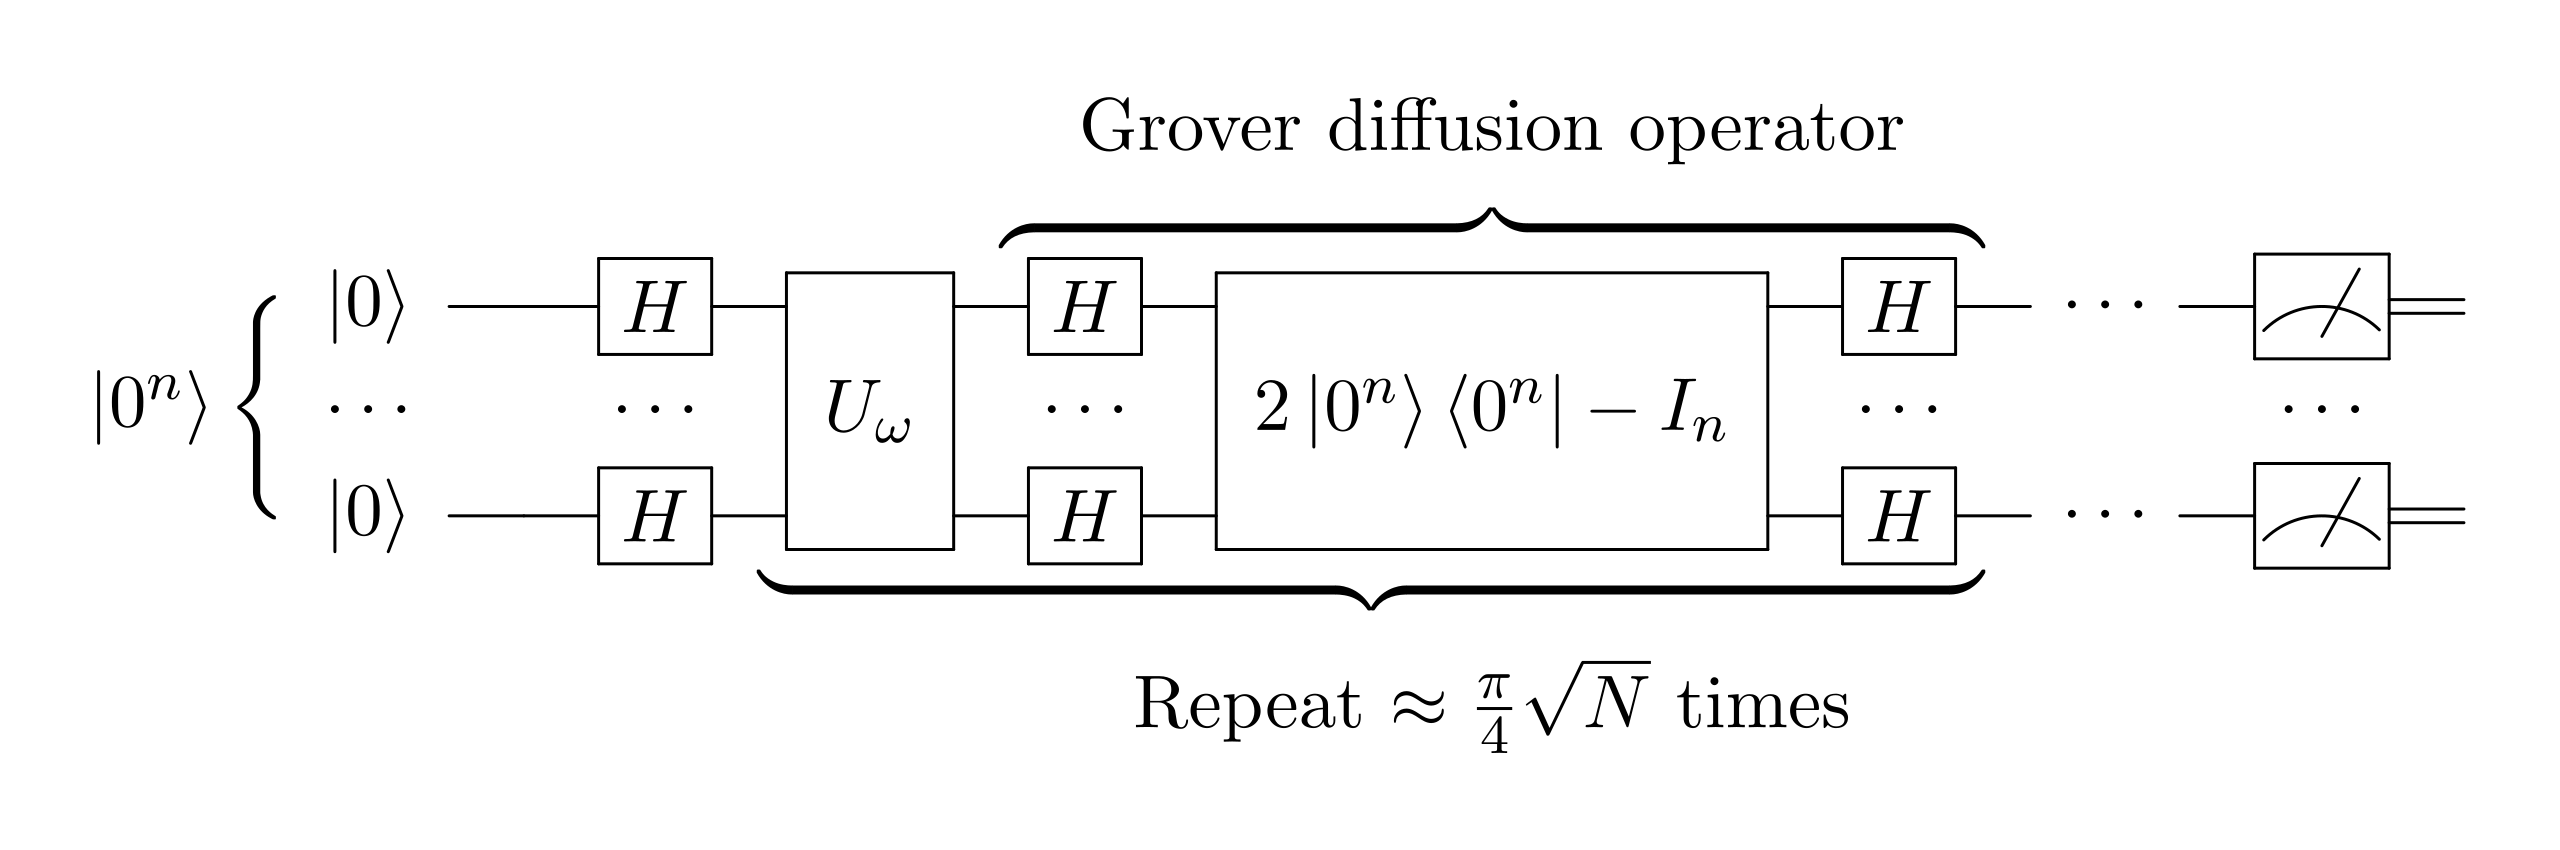
\includegraphics[keepaspectratio, width=15cm, height=15cm]{grover-circuit}

\section{An Oracle for mining Bitcoin Blocks}{}

\subsection{Functions as Unitary Matrices}{}
We can represent a function as a Unitary Matrix. For example, suppose we have a reverse function that reverses the input bits.

\begin{center}
\begin{tabular}{ |c|c|c| } 
 \hline
 a & b & f = $ba$ \\ 
 0 & 0 & 00 \\ 
 0 & 1 & 10 \\ 
 1 & 0 & 01 \\ 
 1 & 1 & 11 \\ 
 \hline
\end{tabular}
\end{center}

We can represent this as a matrix as follows:\\

$
\begin{bmatrix}
& 00 & 01 & 10 & 11\\
00 &1 & 0 & 0 & 0\\
01 & 0 & 0 & 1 & 0\\
10 & 0& 1 & 0 & 0\\
11& 0& 0 & 0 & 1\\
\end{bmatrix}
$\\

\noindent The first row and column are simply labels. The way to interpret this is: 1 marks the answer. So you look at the column for a particular input, say 10 and then look for the row where there's a 1, the row number is the answer. For example, if we look at column 10, there is a 1 at row 01, meaning $f(10) = 01$

\subsection{Reversible Computing}{}
\noindent Quantum computation needs to be reversible. This means that for a given input, a circuit produces some output but, unlike classical computers, we should be able to recover the input from the output. Why is this a requirement?\\

\noindent Rolf Landauer proposed the Landauer principle, which proposes that \textbf{information is physical}. He proposed that fundamentally, logic gates dissipate heat because they are irreversible. Since they are irreversible, they \textbf{delete} information. He proposed that deleting a single bit of information increases a systems entropy and the associated energy is released as heat.\\

\noindent For example, a logical AND gate takes 2 inputs but produces only one output, we cannot recover the original bits, and so we lost or deleted information.  We can think of the information as being conserved, it can't be created or destroyed and so must go somewhere, and it dissipates away as heat.\\

\noindent Landauer proposed that the minimum amount of energy required to delete one bit of information was $K T$ ln (2), where K is the Boltzmann constant and T is the temperature of the system. It was derived from the Boltzmann Entropy Formula which states that $\frac{E}{T} = K ln(W)$ where $E$ is energy and $W$ is the number of states the system can be in. In the case of a bit, it can be in 2 states, 0 or 1 and so $W = 2$ and so we get $E = K T ln(2)$. For $N$ bits, we have $W = 2^{N}$ states which gives $E = K T ln(2^N)$ which is equivalent to $N K T ln (2)$ which shows that the energy dissipated by logic gates scales linearly with the number of bits.\\

\subsection{Reversible Functions}{}


\noindent We can turn an arbitrary non reversible function $f(x)$, into a reversible function by doing $U_{f} (x, h) = (x, h \oplus  f(x))$. \\

\noindent In terms of a matrix representing a function, we can ensure it is reversible by satisfying $U_f \ket{x} = (-1)^{f(x)} \ket{x}$\\

\noindent This means our diagonal contains -1 or 1. $f(x) = 0$ when $x$ is not a solution and $f(x) = 1$ when $x$ is a solution.

 \subsection{Pseudocode}{}
We can use the following Python pseudocode to achieve the above.
\begin{Verbatim}[tabsize=4]
def f(x):	
	if x is a valid nonce:
		return 1
	return 0

def phase(x):
	return (-1)**f(x)

def functionToMatrix(fn, n):
	size = 2**n
	matrix = []
	for i in range(size):
		matrix[i][i] = fn(i)
	return matrix
	
\end{Verbatim} 

\section{Mining Implementation Overview}{}
We have implemented the full mining solution with Grover's Algorithm and tested it on a simulator and it works correctly. To run the program follow this format:

\begin{verbatim}
python main.py n i
\end{verbatim}

\noindent Where $n$ is the number of qubits to use and $i$ is the number of Grover iterations to use, more iterations means our target result is amplified more and has a higher probability. Note that we can't use any $n$ as a potential nonce may be larger than $n$ bits, hence we use the following test block and attempt to find a hash with 2 leading zeros and we know a nonce with 6  bits exist.\\

\noindent Test block:
\begin{verbatim}
block_header = {
    nVersion: 0x1,
    hashPrevBlock: 0x00000000839a8e6886ab5951d76f411475428afc90947ee320161bbf18eb6048,
    hashMerkleRoot: 0x9b0fc92260312ce44e74ef369f5c66bbb85848f2eddd5a7a1cde251e54ccfdd5,
    nTime: 1231467715,
    nBits: 486604799
}
\end{verbatim}

\noindent This block is real data from block number 2 of the Bitcoin blockchain obtained from \href{https://www.blockchain.com/btc/block/2}{here}. We omit the nNonce field as we are trying to search for it.\\

\noindent For this block, the nonce 47 computes a hash with 2 leading zeros. I ran a seperate script to check this. We expect to find 47 as a solution when running our code.\\

\noindent Running the following:

\begin{verbatim}
python main.py 6 5
\end{verbatim}

\noindent Which means $n = 6$ qubits are to be used and 5 iterations of Grover's Algorithm. We get the following results:

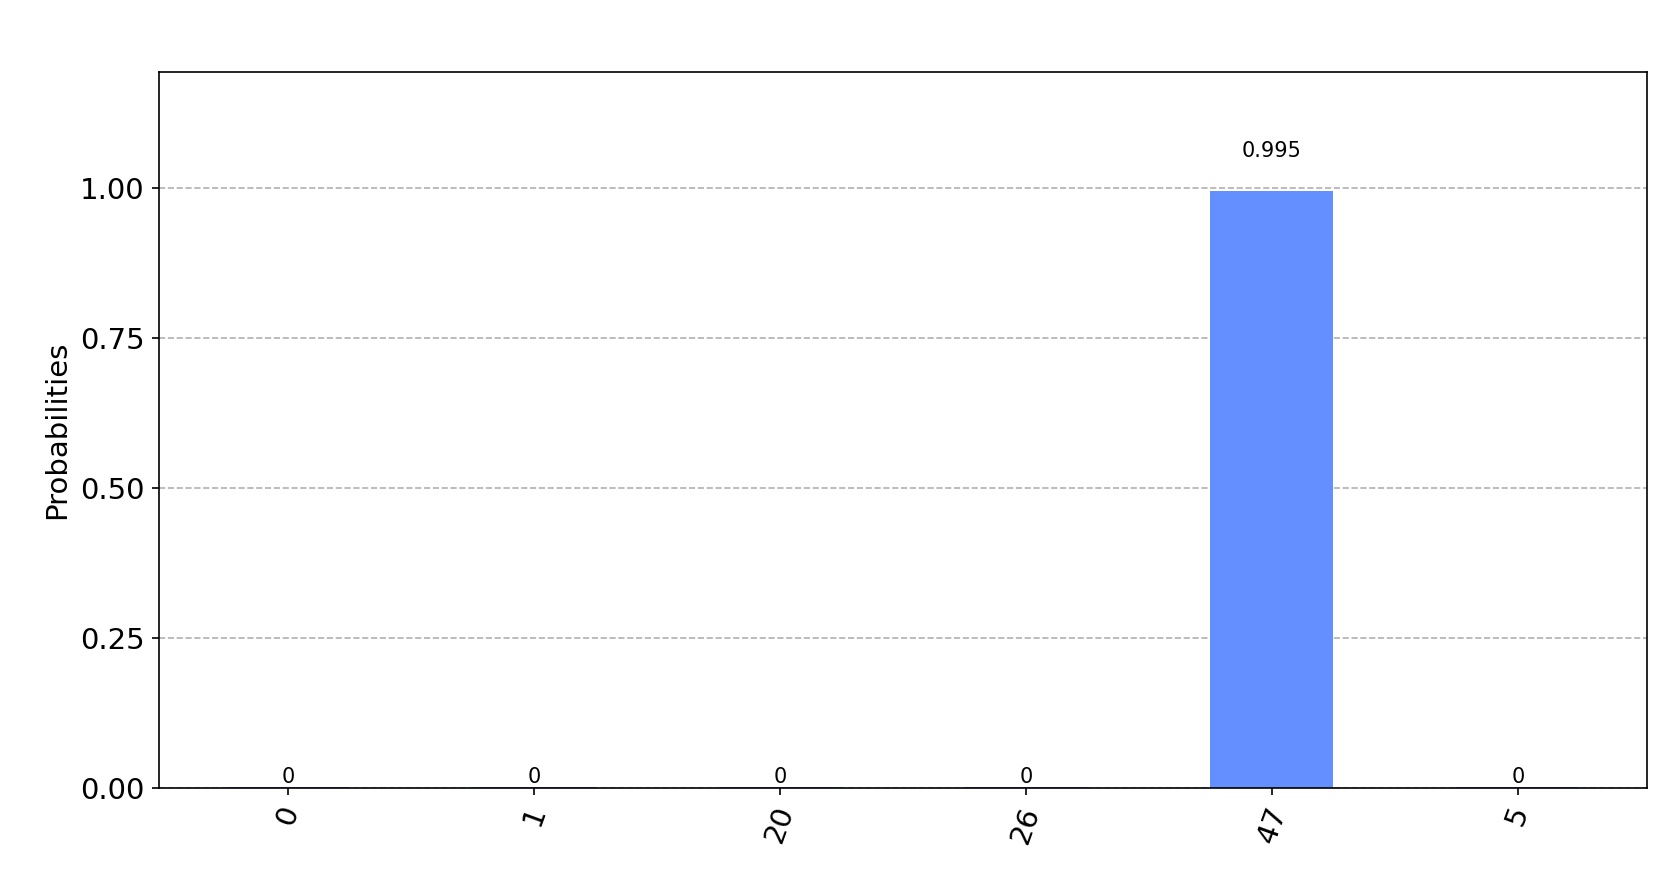
\includegraphics[keepaspectratio, width=15cm, height=15cm]{plot}

We can see that the probability of input 47 is 96.1\%, which is what we expect.

\section{Implementation Analysis and Practical Considerations}{}
The reason we are limited in the earlier section is because the amount of space required to store the Unitary matrix grows exponentially with the number of input bits. For $n$ bits, the space complexity is $O(2^{2n})$. This is because $n$ bits can be in $2^{n}$ states and our matrix must account for each one. \\

\noindent To put this into perspective, even for $n = 20$ bits (which is only 7 digit base-10 number at most), we would need a matrix with a trillion rows and columns! This obviously will not scale. To further illustrate the impracticality of this, the most recently mined block (at the time of writing), block 713463 (found \href{https://www.blockchain.com/btc/block/713463}{here}) had a nonce of 148,510,277 which in binary, is 28 bits, so using our approach we'd need $2^{56}$ entries in our matrix!\\

\noindent I haven't dug deeply into Qiskit internals but, it may be possible to encode only the values on the diagonal of the matrix and then pass it to Qiskit's \lstinline{g.unitary()}. This way, our space complexity would be $O(2^n)$ which is still quite large, but a significant improvement.



\end{document}
